% ===================================================================
%                   Presentación con Latex Beamer
% ===================================================================
\documentclass[9pt,xcolor=svgnames]{beamer}
%\documentclass[handout,xcolor=svgnames]{beamer} %Version imprimible
% -------------------------------------------------------------------
% Paquetes personalizados
\usepackage{../paquetes}
\usepackage{../colores}
\usepackage{../info}
\usepackage{../modo}
% -------------------------------------------------------------------

% Comienza el documento
\begin{document}
% Tikz -> Imágenes
\tikzstyle{every picture}+=[remember picture]
% Entorno matemático
\everymath{\displaystyle}
% -------------------------------------------------------------------
\subtitle{El retorno del proyecto}
\date{Junio 2009}
% -------------------------------------------------------------------
% Fondo blanco: primera página
% ------------------------------------------------------------------

\beamersetaveragebackground{white}

\begin{frame}
 \thispagestyle{empty}
 \begin{figure}[t]
  \centering
  
\includegraphics[scale=0.4]{./Imagenes/logo_cachimba.pdf}

\noindent \Huge Presenta...
\end{figure}
\end{frame}


\begin{frame}
 \thispagestyle{empty}
 
 \animate<2-3> 
 \begin{figure}[t]
  \centering
  \includegraphics<1>[scale=0.7]{../Imagenes/logo_1.pdf}
  \includegraphics<2>[scale=0.7]{../Imagenes/logo_2.pdf}
  \includegraphics<3>[scale=0.7]{../Imagenes/logo_3.pdf}
  \includegraphics<4>[scale=0.7]{../Imagenes/logo_4.pdf}
 \end{figure}
\end{frame}


% -------------------------------------------------------------------
% Fondo para el resto del documento
\setbeamertemplate{background}{

\includegraphics[width=\paperwidth,height=\paperheight]
{../Imagenes/fondo.pdf}
}
% -------------------------------------------------------------------


% Continuación:
% Transparencia de Inicio -> Título
\begin{frame}
 \titlepage
\end{frame}

\normalsize

% Transparencia de índice
\begin{frame}{Índice} 
 \transdissolve
 \tableofcontents
\end{frame}
  
  
 \section{Estado del proyecto}
 
  \subsection{Actualización de la planificación}
  
  \begin{frame}{Diagrama de Gannt}
   
   \begin{figure}[t]
    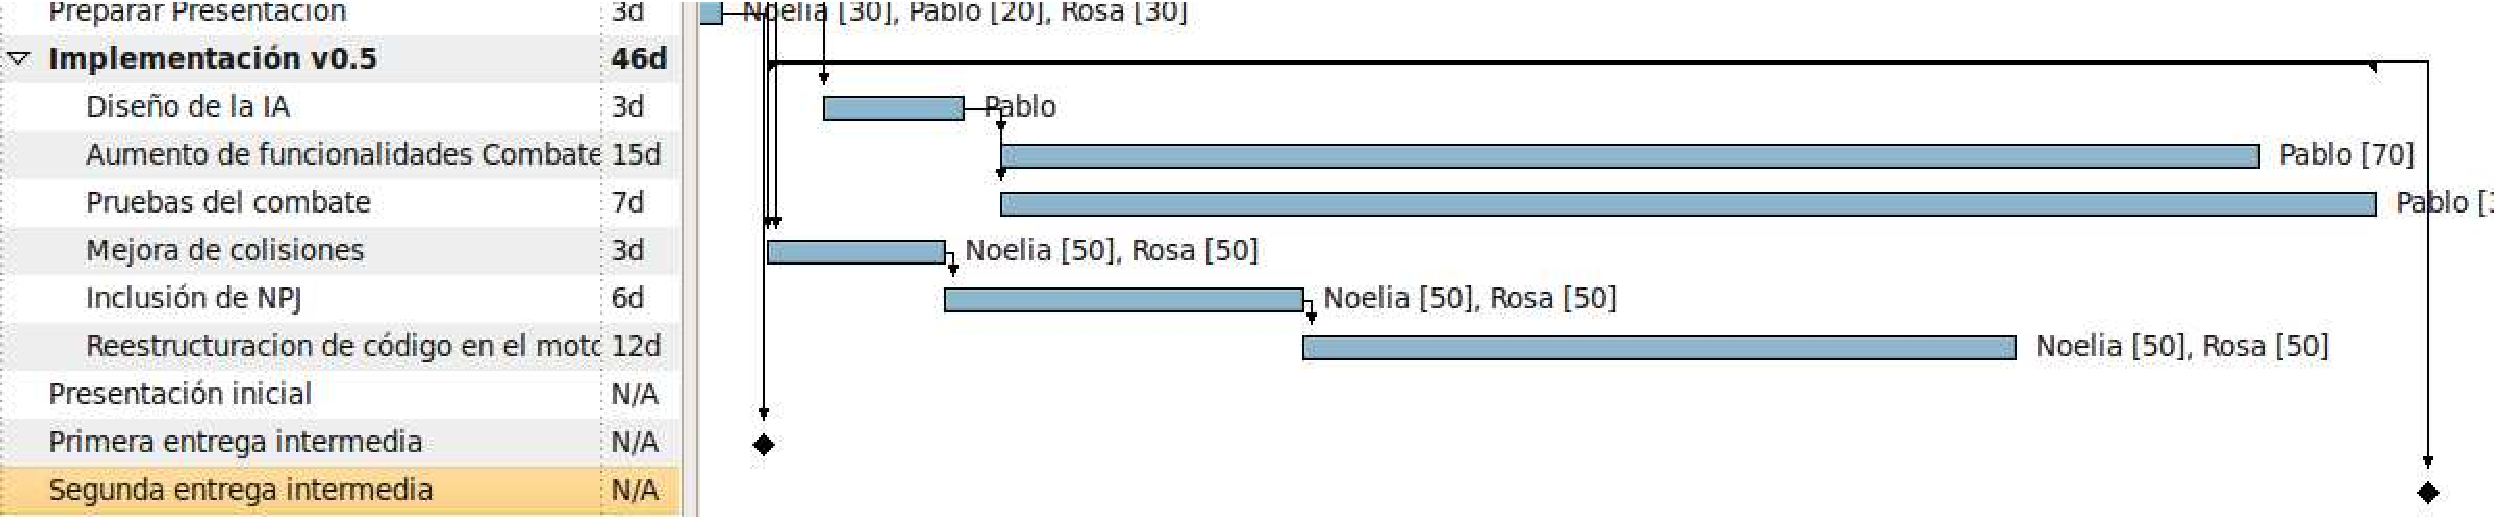
\includegraphics[scale=0.225]{./Imagenes/gannt.pdf}
   \end{figure}
   
  \end{frame}
   
   
   
   \subsection{Modificaciones sufridas por el proyecto}
   
   \begin{frame}{Modificaciones y justificaciones}
    
    \begin{itemize}
     \item Desde la anterior presentación no hemos considerado
	   ninguna modificación del proyecto inicial, por lo
	   estamos siguiendo el plan inicial.
	 
    \end{itemize}    
    
   \end{frame}
   
   
 \section{Presentación Previa del producto}

 \subsection{Menu principal}
 \begin{frame}{Estado del menu principal}
   \begin{figure}[t]
    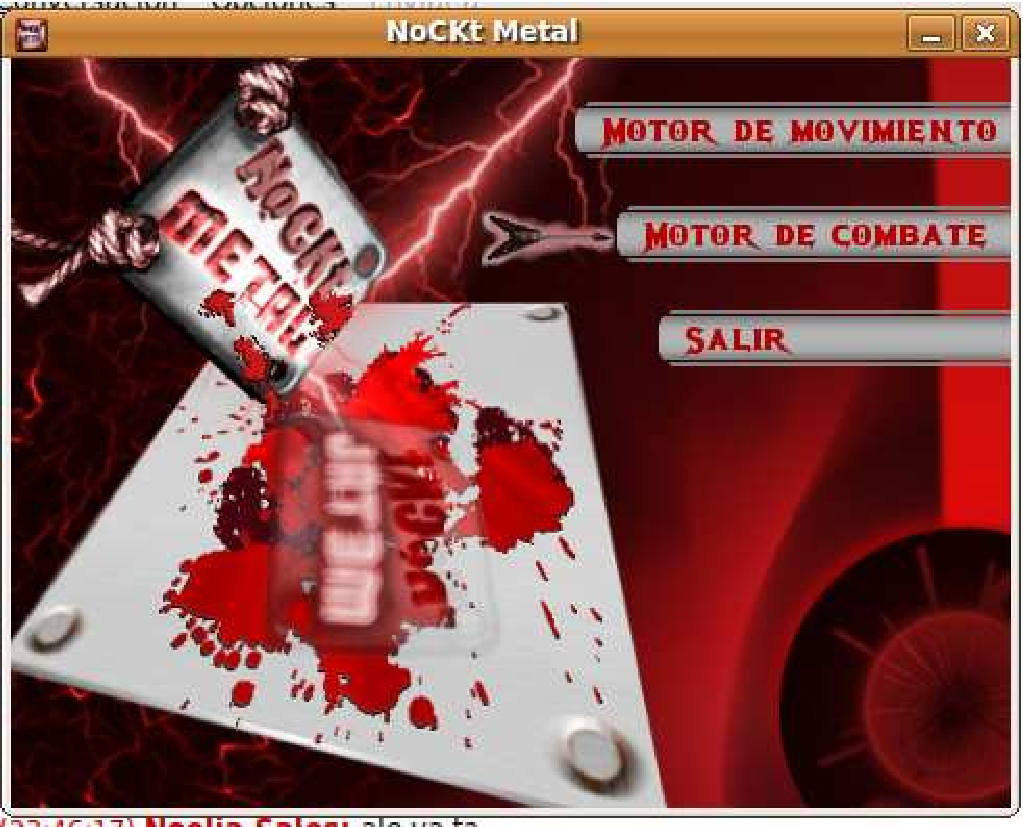
\includegraphics[scale=0.35]{./Imagenes/menu.pdf}
   \end{figure}
 \end{frame}
 
   \subsection{Producto actual}

   \begin{frame}{Estado actual: Motor de Combate}
    \begin{itemize}
     \item Inclusión de una simple IA para los rivales
     \item Mejora de la serialización de los objetos, añadiendo
	   construcciones desde ficheros.
     \item Adquisición de experiencia de los PJs
     \item Más grupos enemigos con distintas cualidades cada uno.
     \item Clase \texttt{Biblioteca} que indexa los datos para 
	   guardados de partida.
     \item Solucionados algunos bugs críticos
    \end{itemize}
   \end{frame}

   \begin{frame}{Captura de pantalla: Motor de combate}
   \begin{figure}[t]
    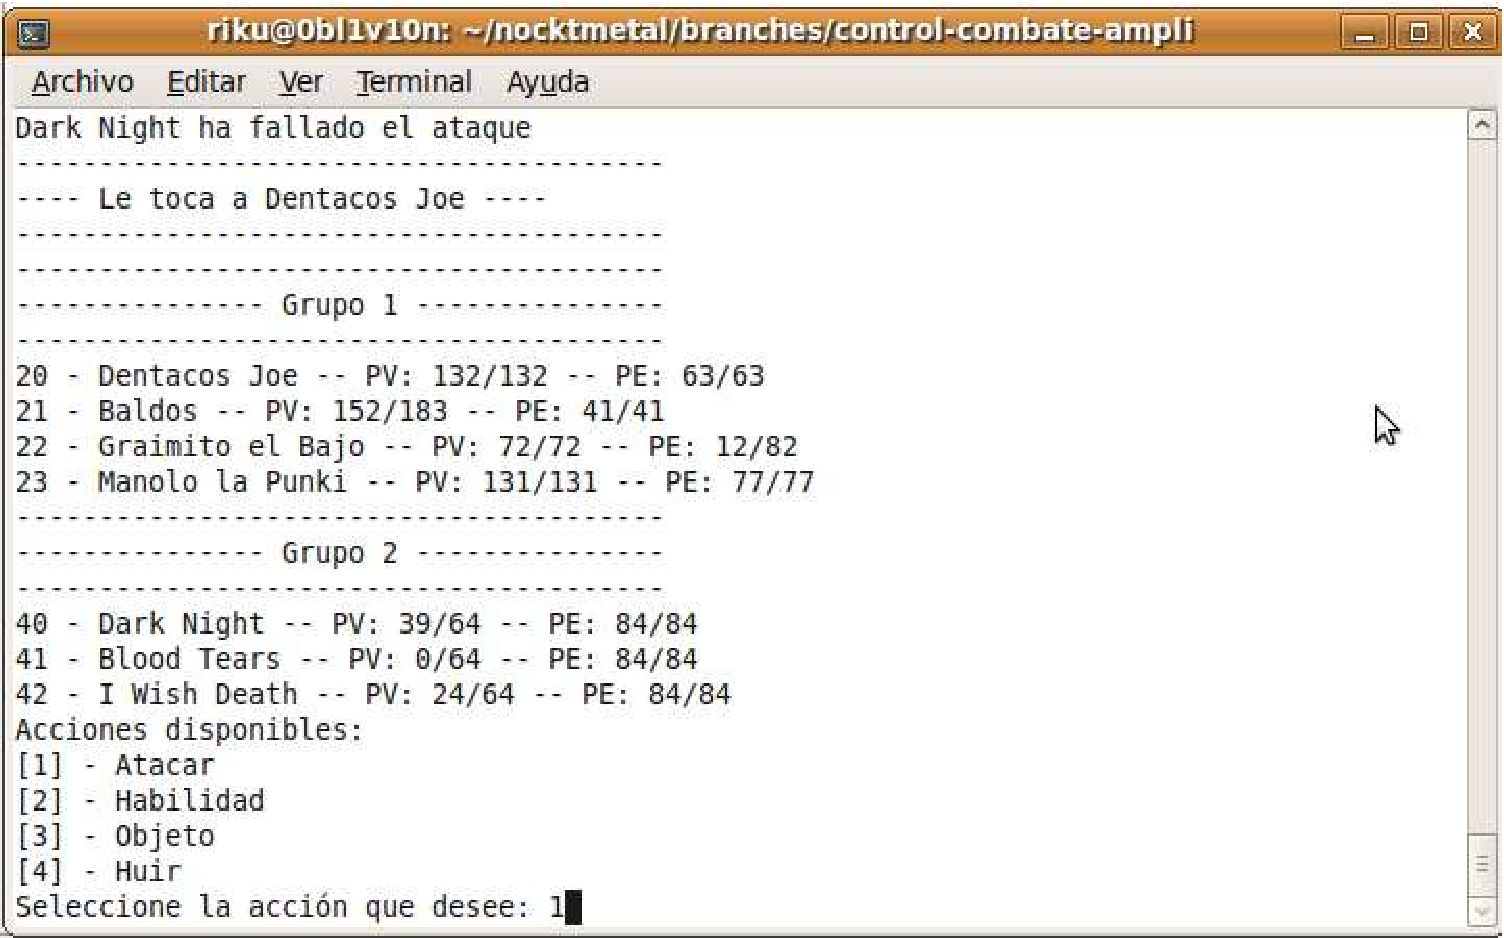
\includegraphics[scale=0.35]{./Imagenes/combate.pdf}
   \end{figure}    
   \end{frame}

   \begin{frame}{Estado actual: Motor de movimiento}
    \begin{itemize}
     \item Añadidos NPJs en el motor, ampliando la funcionalidad del mismo.
     \item Añadidas las funcionalidades de diálogos entre PJs y NPJs.
     \item Tratamiento de eventos para futura interaccion entre PJs y
	   NPJs u objetos
     \item Mejora de las colisiones en el mapa, detectando además los NPJ
     \item Solucionados algunos bugs y re-escritura de algunas clases
	   para una mejor cohesión
     \item Menu inicial :)
    \end{itemize}
   \end{frame}


   \begin{frame}{Captura de pantalla: Motor gráfico}
   \begin{figure}[t]
    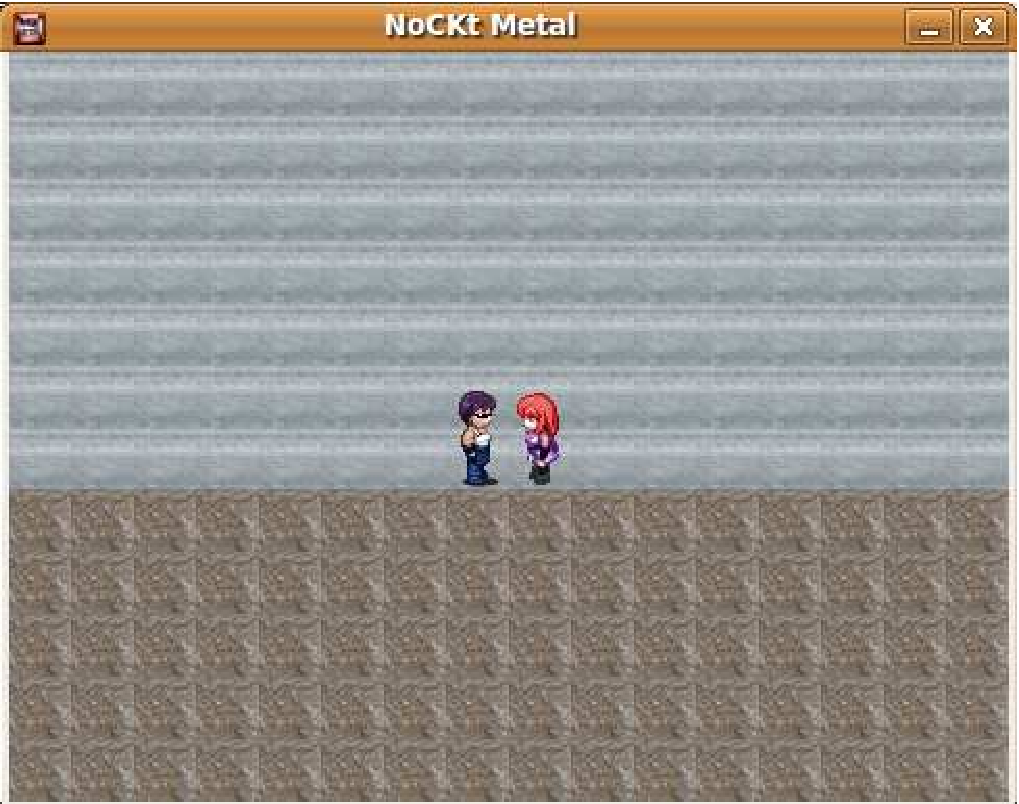
\includegraphics[scale=0.35]{./Imagenes/movimiento.pdf}
   \end{figure}    
   \end{frame}

   \subsection{Inteligencia Artificial}
   \begin{frame}
     La IA solo es utilizada en el motor de combate, y no es una IA
     demasiado crítica, ya que no tiene que actuar en tiempo real, y
     las variables de decisión no son demasiado complejas.\\

     Por ahora, solo realiza ataques simples. En la próxima versión hará
     ataques, usará objetos e incluso puede que intente huir.\\

     \begin{block}{Secuencia}
       \begin{itemize}
       \item Comprueba el porcentaje de vida de cada rival.
       \item Asigna una puntuación en función del porcentaje de vida,
         de forma que el que tiene menos vida, tiene una puntuación más alta.
       \item Se realiza una tirada pseudo-aleatoria, de forma que los
         que tienen menos vida es más posible que sean atacados que el resto.
       \end{itemize}
     \end{block}
   \end{frame}
   

 \section{Calidad de la implementación}
 
  \subsection{Calidad del código}
  
  \begin{frame}{Implementación de código en grupo}
   A continuación veremos unos ejemplos de códigos que forman parte del
   proyecto.

   \begin{block}{Elección de los códigos a mostrar}
    En representación de todos los códigos que contiene el proyecto,
    hemos escogido dos ejemplos en los cuales se sustenta la base de
    cualquier juego: el personaje principal.\\

    \vspace*{0.3cm}    
    Hemos incluido las clases que abstraen el personaje desde los dos
    puntos de vista:
    \begin{description}
     \item[Clase combatiente:] base del motor de combate\\
		Representación de una clase cualquiera
     \item[Clase Personaje:] base del motor de movimiento\\
		Representación de una clase desarrollada
		``simultáneamente'' por varios componentes
    \end{description}
   \end{block}
  \end{frame}
 
  \subsection{Ejemplo: Clase (estructura en objetos)}
  
  
  \begin{frame}[fragile=singleslide]{Ejemplo: Clase \textbf{Combatiente} (1)}
   
   \begin{lstlisting}[style=C++]
    #ifndef _COMBATIENTE_H
    #define _COMBATIENTE_H
    
    #include ...

    class Combatiente: public Atributos {
     public:
      class AtaqueFallado: public std::exception {
        public:
        const char* what() const throw () {
          return "El ataque ha fallado!";
        }
      };

      Combatiente(std::string nombre, Uint32 id,
                  AtributoBase atr, Grupo &grupo,
                  std::pair<Uint32, Uint32> rangoArma,
                  string rXML, Uint32 exp = 0, Uint32 exp_ganable = 0, 
                  Uint32 aciertoArma = 15, Uint32 armadura = 20);
   \end{lstlisting}
    
  \end{frame}
    
  \begin{frame}[fragile=singleslide]{Ejemplo: Clase \textbf{Combatiente} (2)}
   \begin{lstlisting}[style=C++]                  
      Combatiente(const char* ruta_XML) {
        cargar_XML(*this, ruta_XML);
      }

      /*--- METODOS GETTER --- */
      /* ..................... */

      Uint32 tiradaArma() const {
        Aleatorio a;
        return a.valorEntero(_rangoArma.first, _rangoArma.second);
      }
      void addHabilidad(Habilidad& h);
      Uint32 ataqueSimple(Combatiente &objetivo) throw(AtaqueFallado);
      Uint32 usarObjeto(Uint32 i, Combatiente& objetivo) throw (Inventario::ObjetoNoEnInventario, Objeto::CantidadItemInsuficiente);
      Uint32 ataqueEspecial(Uint32 i, Combatiente& objetivo);   
   \end{lstlisting}
   
  \end{frame}
  \begin{frame}[fragile=singleslide]{Ejemplo: Clase \textbf{Combatiente} (3)}
   \begin{lstlisting}[style=C++]
      void actualizarXML() {
        guardar_XML(*this, _ruta_XML.c_str());
      }

     private:
       std::string _nombre;
       Uint32 _idCombatiente
       std::map<Uint32, Habilidad*> _habilidades;
       Inventario *_inventario;
       Grupo* _grupo;
       bool _pasarTurno;
       Uint32 _experienciaGanable;
       std::pair<Uint32, Uint32> _rangoArma;
       Uint32 _aciertoArma;
       Uint32 _armadura;
       friend class boost::serialization::access;

       template<class Archive>
       void serialize(Archive & ar, const unsigned int version)
#endif
   \end{lstlisting}
 \end{frame}
  
  \subsection{Ejemplo: Interfaz principal entre clases}
  \begin{frame}[fragile=singleslide]{Ejemplo: Clase \textbf{Personaje} (1)}
   
   \begin{lstlisting}[style=C++]
#ifndef _PERSONAJE_
#define _PERSONAJE_

#include ...

class Personaje {
public:

    Personaje();
    Personaje(Uint32 i, Uint32 x, Uint32 y, Pantalla* p, const char* sprite,
                     Uint32 f = 4, Uint32 c = 4);               
    Personaje(Uint32 i, Uint32 x, Uint32 y, Uint32 tam, Pantalla* p,
              const char* sprite, Uint32 f = 4, Uint32 c = 4);       
    Personaje(Uint32 i, Uint32 x, Uint32 y, Uint32 mapax, Uint32 mapay,
              Uint32 tam, Pantalla* p, const char* sprite, Uint32 f = 4,
              Uint32 c = 4);
    ~Personaje();


   \end{lstlisting}
  \end{frame}
  
  \begin{frame}[fragile=singleslide]{Ejemplo: Clase \textbf{Personaje} (2)}
   
   \begin{lstlisting}[style=C++]
    /*--- METODOS GETTER --- */
    /* ..................... */

    void setPosicion(Uint32 x, Uint32 y);
    void setPosicion();
    void setRango(Uint16 margenIzdo, Uint16 margenArriba, Uint16 rangoAncho,
                  Uint16 rangoAlto);
    void setRango(Uint16 rangoAncho = 0, Uint16 rangoAlto = 0);
    void setMapa(Uint16 x, Uint16 y);
    void setVelocidad(Uint16 v);

    void subirEnMapa();
    void bajarEnMapa();
    void izdaEnMapa();
    void dchaEnMapa();

    void subirEnPantalla();
    void bajarEnPantalla();
    void izdaEnPantalla();
    void dchaEnPantalla();
   \end{lstlisting}
  \end{frame}

  \begin{frame}[fragile=singleslide]{Ejemplo: Clase \textbf{Personaje} (3)}
   
   \begin{lstlisting}[style=C++]
    void dibujarPosicionFrente();
    void dibujarPosicionEspaldas();
    void dibujarPosicionLatIzda();
    void dibujarPosicionLatDcha();    
    void moverArriba(Uint32 mov, Uint32 desp = 0);
    void moverAbajo(Uint32 mov, Uint32 desp = 0);
    void moverIzda(Uint32 mov, Uint32 desp = 0);
    void moverDcha(Uint32 mov, Uint32 desp = 0);

protected:
    void mover(Uint32 movimiento, Uint32 secuencia);
    Uint32 _id, _mapaX, _mapaY, _x, _y, _pantX, _pantY, _tam, _velocidad;
    vector<Uint32> _desp;
    SDL_Rect _rango;
    Pantalla* _p;
    Sprite _sprite;
};
    /*--- METODOS INLINE --- */
    /* ..................... */

#endif
   \end{lstlisting}
  \end{frame}
    
  


 \section{Conclusión}
 
  \subsection{Solución de problemas}

  \begin{frame}{Problemas y soluciones}
   \begin{itemize}
    \item Ordenación del vector en los turnos
    \item Utilización de vectores de bajo nivel fallaba varias
     veces.
	  \begin{description}
	   \item[Solución:] \texttt{std::vector<>}
	  \end{description}
    \item IA totalmente aleatoria: ponderación por porcentaje de vida.
    \item Fechas en la que nos encontramos.
	  \begin{description}
	   \item[Solución:] Retrasar plazos
	  \end{description}
    \item Problema en capas \texttt{SDL\_Surface}.
	  \begin{description}
	   \item[Solución:] Redibujado de algunas capas en una
		       sola
	  \end{description}
    \item Aceleración del menú inicial debido a un redibujado de los
	  elementos del mismo.	  
	  \begin{description}
	   \item[Solución:] Dibujar los elementos una única vez
	  \end{description}
   \end{itemize}

  
  \end{frame}

  \begin{frame}{Conclusión final}
   A pesar de los problemas de tiempo y los inconvenientes sufridos el
   proyecto avanza.\\

   Se han solventado los problemas más serios y se intenta unificar los
   dos motores que ya poseen una base sólida.
  \end{frame}
  
  
 \section{Para terminar}
  
\scriptsize

 \begin{frame}{Esta presentación es libre}
  Copyright 2009 Noelia Sales Montes\\
  Parte del Proyecto NoCKt Metal\\
  \url{http://nocktmetal.forja.rediris.es/}
  
  \vspace*{0.3cm}
  
  Creative Commons Attribution License
  \url{http://creativecommons.org/licenses/by/2.0/}\\
  Creative Commons, 559 Nathan Abbott Way, Stanford, California 94305,
  USA.
  
  \vspace*{0.3cm}
  
  Este trabajo se publica bajo la siguiente licencia:\\
  Creative Commons Attribution License
  \url{http://creativecommons.org/licenses/by/3.0/}
  
  \vspace*{0.3cm}
  
  Usted es libre de:
  \begin{itemize}
   \item copiar, distribuir y comunicar públicamente la obra
   \item hacer obras derivadas
  \end{itemize}
  
  Bajo las condiciones siguientes:
  \begin{itemize}
   \item Reconocimiento. Debe reconocer los créditos de la obra de la
	 manera especificada por el autor o el licenciador (pero no de una
	 manera que sugiera que tiene su apoyo o apoyan el uso que hace de
	 su obra).
   \item Al reutilizar o distribuir la obra, tiene que dejar bien claro los
	 términos de la licencia de esta obra.
   \item Alguna de estas condiciones puede no aplicarse si se obtiene el
	 permiso del titular de los derechos de autor
   \item Nada en esta licencia menoscaba o restringe los derechos morales
	 del autor.
  \end{itemize}
 \end{frame}


  
\end{document}
 
